% =============================================================================
% Module 10: Strong Lensing by Galaxy Clusters
% =============================================================================
% Sources: Congdon & Keeton Ch. 7, Narayan & Bartelmann Sec. 4,
%          Meneghetti 2021 Ch. 5
% Mathematica: ../Mathematica/10_Cluster_Lensing/
% =============================================================================

\chapter{Strong Lensing by Galaxy Clusters}
\label{ch:cluster_lensing}

\begin{quote}
\textit{Galaxy clusters are the most massive gravitationally bound objects
in the universe.  When they act as gravitational lenses, they produce the
most dramatic manifestations of general relativity visible in the sky:
giant luminous arcs stretching tens of arcseconds, dozens of multiply
imaged background galaxies, and magnification factors large enough to
reveal individual stars at cosmological distances.}
\hfill --- adapted from Meneghetti (2021)
\end{quote}

\noindent
This final module brings together the entire gravitational lensing
framework developed in Modules~1--9 and applies it to the most
spectacular setting: \textbf{galaxy clusters}.  Where a single galaxy
lens (Module~9) typically produces two or four images of a background
source with an Einstein radius of $\sim 1''$, a massive galaxy cluster
can produce dozens of multiple image systems, giant arcs with
length-to-width ratios exceeding 10:1, and Einstein radii of
$\sim 10''$--$50''$.

Galaxy clusters have total masses of $10^{14}$--$10^{15}\,\Msun$,
with $\sim 85\%$ in dark matter, $\sim 13\%$ in hot intracluster gas,
and only $\sim 2\%$ in stars.  Their mass distributions are
well-described by the NFW profile introduced in
Module~\ref{ch:axisymmetric_models}, now applied at scales 100--1000
times more massive than individual galaxy halos.  The richness of
cluster lensing --- many image systems at multiple source redshifts ---
provides powerful constraints on the dark matter distribution and on
cosmological parameters.

\medskip
\noindent
\textbf{Companion Mathematica files:}
\begin{itemize}[nosep]
    \item \mathlink{10_Cluster_Lensing/cluster\_lensing.wl}{cluster\_lensing.wl}
          --- NFW cluster lensing quantities; critical curves and
          caustics at cluster scale; ray-tracing through cluster
          potential to generate arcs; Einstein radius vs.\ cluster mass;
          figures exported to \texttt{Figures/10\_Cluster\_Lensing/}
    \item \mathlink{10_Cluster_Lensing/nfw\_cluster.nb}{nfw\_cluster.nb}
          --- interactive notebook with \texttt{Manipulate} widgets for
          NFW cluster parameters, giant arc formation, magnification
          maps, and weak lensing shear profiles
\end{itemize}


% =====================================================================
\section{Introduction: Why Cluster Lensing Is Special}
\label{sec:cluster_intro}

Galaxy clusters occupy a unique place in both astrophysics and
gravitational lensing.  They are the largest objects in the universe
whose properties are determined by gravity alone --- they sit at the
top of the hierarchy of cosmic structure.  Their enormous masses make
them the most powerful gravitational lenses, producing phenomena that
are qualitatively different from galaxy-scale lensing:

\begin{enumerate}
    \item \textbf{Giant arcs.}  Extended background galaxies are
          stretched into luminous arcs tens of arcseconds long, tracing
          out the tangential critical curve of the cluster potential.
          The first giant arc was discovered in Abell~370 by Soucail
          et al.\ (1987), confirming the gravitational lensing
          interpretation of these features.

    \item \textbf{Many multiple image systems.}  A single massive
          cluster can produce 10--30 or more distinct sets of multiple
          images, each from a different background galaxy at a different
          redshift.  Each set independently constrains the cluster mass
          model.

    \item \textbf{Extreme magnification.}  Magnification factors of
          $\mu \sim 10$--100 are common near the critical curves of
          clusters.  This turns clusters into ``gravitational
          telescopes'' that reveal galaxies and even individual stars
          at redshifts $z > 6$ that would otherwise be undetectable.

    \item \textbf{Sensitivity to dark matter.}  Because clusters are
          dark-matter dominated, their lensing signal directly probes
          the dark matter distribution --- its radial profile,
          substructure, and overall mass.

    \item \textbf{Cosmological probe.}  The abundance and properties
          of cluster lenses depend on cosmological parameters
          ($\Omegam$, $\sigma_8$, the dark energy equation of state),
          making cluster lensing a tool for precision cosmology.
\end{enumerate}


% =====================================================================
\section{NFW Model for Cluster Lensing}
\label{sec:nfw_cluster}

In Module~\ref{ch:axisymmetric_models} (Section~\ref{sec:nfw}) we
introduced the NFW density profile as the universal dark matter halo
profile.  Here we apply it at \textbf{cluster scale}, where the
relevant parameters are much larger than for galaxy halos.

\subsection{Cluster-Scale NFW Parameters}

The NFW profile (eq.~\ref{eq:nfw_rho}) is parametrized by the virial
mass $M_{200}$ and concentration $c = r_{200}/r_s$.  Typical values
for galaxy clusters are:
\begin{center}
\begin{tabular}{lcc}
\toprule
\textbf{Parameter} & \textbf{Galaxy halo} & \textbf{Cluster halo} \\
\midrule
$M_{200}$ & $10^{12}\,\Msun$ & $10^{14}$--$10^{15}\,\Msun$ \\
$c$ & $10$--$20$ & $3$--$8$ \\
$r_s$ & $15$--$30$ kpc & $200$--$500$ kpc \\
$r_{200}$ & $200$--$300$ kpc & $1$--$2$ Mpc \\
\bottomrule
\end{tabular}
\end{center}
The key difference is that clusters are \textit{less concentrated}
($c \sim 3$--$8$) than galaxy halos ($c \sim 10$--$20$), reflecting
their later formation epoch in the hierarchical structure formation
scenario.  Despite the lower concentration, the vastly greater mass
more than compensates, producing far stronger lensing.

\subsection{Lensing Quantities at Cluster Scale}

The NFW convergence, deflection angle, and shear from
Module~\ref{ch:axisymmetric_models} (eqs.~\ref{eq:nfw_kappa}--\ref{eq:nfw_gamma})
apply directly.  We collect the key formulae here for reference.  Define
$x = \theta/\theta_s$, where $\theta_s = r_s/\Dd$ is the angular scale
radius.  Then:
\begin{align}
    \kappab(x) &= \kappa_s\, f(x) \,,
    \label{eq:cl_nfw_kappa} \\
    \alpha(x) &= \frac{4\kappa_s\,\theta_s}{x}
    \left[\ln\frac{x}{2} + g(x)\right] \,,
    \label{eq:cl_nfw_alpha} \\
    |\gammaL(x)| &= \bar{\kappa}(x) - \kappab(x) \,,
    \label{eq:cl_nfw_gamma}
\end{align}
with the functions $f(x)$ and $g(x)$ defined in
eqs.~\eqref{eq:nfw_f}--\eqref{eq:nfw_g}, and the characteristic
convergence:
\begin{equation}
    \kappa_s = \frac{2\rho_s\, r_s}{\Sigmacr} \,.
    \label{eq:cl_kappa_s}
\end{equation}

\begin{example}
\textbf{Characteristic convergence for a massive cluster.}
For a cluster with $M_{200} = 10^{15}\,\Msun$, $c = 5$, at
$z_d = 0.3$ lensing a source at $z_s = 2$
($\Dd \approx 900$~Mpc, $\Ds \approx 1750$~Mpc,
$\Dds \approx 1400$~Mpc):
\begin{itemize}[nosep]
    \item $r_{200} \approx 2.0$~Mpc, $r_s = r_{200}/c \approx 400$~kpc,
    \item $\theta_s = r_s / \Dd \approx 92''$,
    \item $\kappa_s \approx 0.46$.
\end{itemize}
Since $\kappa_s \times f(x)$ can exceed unity for $x \lesssim 0.5$
(i.e., $\theta \lesssim 46''$), the cluster is a strong lens ---
it has a region where $\kappab > 1$.  These values are computed and
verified in
\mathlink{10_Cluster_Lensing/cluster\_lensing.wl}{cluster\_lensing.wl}.
\end{example}

\subsection{Critical Curves and Caustics for Cluster NFW}
\label{sec:cluster_crit}

For the circularly symmetric NFW profile, the tangential and radial
critical curves are circles.  The tangential critical curve occurs
where $\bar{\kappa}(x) = 1$, i.e.:
\begin{equation}
    \frac{4\kappa_s}{x_t^2}\left[\ln\frac{x_t}{2} + g(x_t)\right] = 1 \,,
    \label{eq:cl_tangential_crit}
\end{equation}
and the radial critical curve where
$2\kappab(x_r) - \bar{\kappa}(x_r) = 1$, i.e.:
\begin{equation}
    2\kappa_s\, f(x_r)
    - \frac{4\kappa_s}{x_r^2}\left[\ln\frac{x_r}{2} + g(x_r)\right] = 1 \,.
    \label{eq:cl_radial_crit}
\end{equation}
Both equations must be solved numerically.  For the cluster parameters
above ($M_{200} = 10^{15}\,\Msun$, $c = 5$, $z_d = 0.3$, $z_s = 2$),
the tangential critical curve has a radius of
$\theta_t \approx 35''$--$40''$, which corresponds to a physical
radius of $\sim 150$~kpc at the cluster redshift.

\begin{remark}
The tangential critical curve radius is often called the
\textbf{Einstein radius} of the cluster, $\thetaE$.  For a cluster,
$\thetaE \sim 10''$--$50''$, compared to $\sim 1''$ for a galaxy
lens.  The enclosed projected mass within $\thetaE$ is of order
$10^{13}$--$10^{14}\,\Msun$ --- the mass of a large galaxy group.
\end{remark}

\subsection{Einstein Radius Scaling with Cluster Mass}

The Einstein radius of an NFW cluster depends on mass, concentration,
and the lens/source redshift configuration.  For a fixed concentration
and redshift configuration, the scaling is approximately:
\begin{equation}
    \thetaE \propto M_{200}^{1/3} \,,
    \label{eq:cl_thetaE_scaling}
\end{equation}
which arises because $\thetaE \sim r_{200}/\Dd$ and
$r_{200} \propto M_{200}^{1/3}$ (from the definition
$M_{200} = (4\pi/3)\, 200\,\rho_{\mathrm{crit}}\, r_{200}^3$).
The actual relationship is more complex due to the dependence of
$\kappa_s$ on $c$ and the nonlinear solution of
eq.~\eqref{eq:cl_tangential_crit}, but the cube-root scaling provides
a useful approximation.

\begin{figure}[ht]
    \centering
    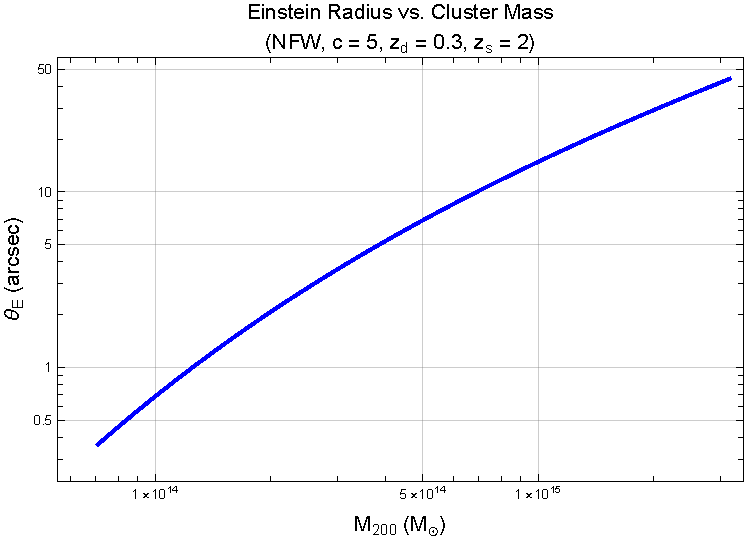
\includegraphics[width=0.75\textwidth]{../Figures/10_Cluster_Lensing/einstein_radius_vs_mass.pdf}
    \caption{Einstein radius $\thetaE$ as a function of cluster mass
    $M_{200}$ for an NFW profile with $c = 5$, $z_d = 0.3$, and
    $z_s = 2$.  The dashed line shows the approximate $M^{1/3}$
    scaling.  Clusters below $M_{200} \sim 10^{14}\,\Msun$ have
    Einstein radii comparable to galaxy-scale lenses.  Generated by
    \texttt{cluster\_lensing.wl}.}
    \label{fig:einstein_radius_vs_mass}
\end{figure}


% =====================================================================
\section{Giant Arcs}
\label{sec:giant_arcs}

Giant luminous arcs are the most visually striking signature of cluster
strong lensing.  They were first discovered by Lynds \& Petrosian (1986)
and Soucail et al.\ (1987) in the clusters Abell~370 and Cl~2244-02,
and their interpretation as gravitationally lensed images of background
galaxies was confirmed spectroscopically by Soucail et al.\ (1988).

\subsection{Formation Mechanism}

Giant arcs form when an extended background galaxy lies close to the
\textbf{tangential caustic} of the cluster.  From the theory of
critical curves (Module~\ref{ch:elliptical_models},
Section~\ref{sec:giant_arcs}):
\begin{enumerate}
    \item The source galaxy is near (but not exactly on) the tangential
          caustic in the source plane.
    \item Its images lie near the tangential critical curve in the image
          plane, where $\lambda_- \approx 0$.
    \item The images are stretched \textit{tangentially} (along the
          critical curve) by a large factor
          $\mu_{\mathrm{tan}} \propto 1/\sqrt{d_\perp}$, where
          $d_\perp$ is the perpendicular distance from the caustic.
    \item The radial magnification remains of order unity, so the
          image is a thin, elongated \textbf{arc} that traces the
          critical curve.
\end{enumerate}

\subsection{Ray-Tracing Through a Cluster Potential}
\label{sec:ray_trace}

To visualize arc formation, we \textbf{ray-trace} an extended source
through the cluster lens equation.  The procedure is:
\begin{enumerate}
    \item Define the source as a set of points in the source plane,
          e.g., a circular disk of angular radius $\beta_0$ centered
          at position $\vecbeta_0$.
    \item For each source point $\vecbeta$, solve the lens equation
          $\vecbeta = \vectheta - \vecalpha(\vectheta)$ for all
          image positions $\vectheta$.  For a cluster, this is done
          numerically on a fine grid.
    \item Plot the union of all image positions to obtain the lensed
          image of the source.
\end{enumerate}

In practice, it is more efficient to use the \textbf{inverse
ray-tracing} approach: for each pixel $\vectheta$ in the image
plane, compute $\vecbeta = \vectheta - \vecalpha(\vectheta)$ and
check whether $\vecbeta$ falls within the source.  If it does,
that pixel is part of a lensed image.

\begin{figure}[ht]
    \centering
    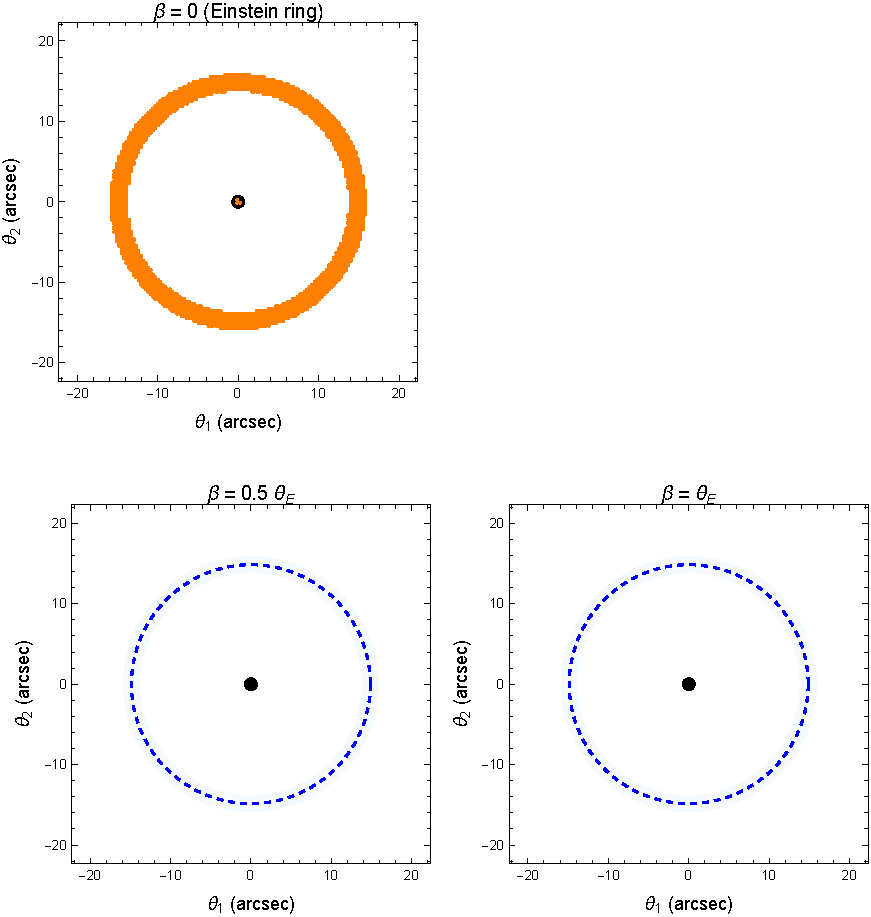
\includegraphics[width=0.85\textwidth]{../Figures/10_Cluster_Lensing/giant_arc_formation.pdf}
    \caption{Giant arc formation by an NFW cluster
    ($M_{200} = 10^{15}\,\Msun$, $c = 5$, $z_d = 0.3$, $z_s = 2$).
    A circular source of radius $0.5''$ is placed at three positions:
    $\beta = 0$ (Einstein ring, left), $\beta = 0.5\,\thetaE$
    (giant arc, center), and $\beta = \thetaE$ (near the critical
    curve, right).  The critical curve is shown as a dashed circle.
    Generated by \texttt{cluster\_lensing.wl}.}
    \label{fig:giant_arc_formation}
\end{figure}

\subsection{Length-to-Width Ratio}

The \textbf{length-to-width ratio} (or axis ratio) of an arc is a
direct measure of the tangential magnification:
\begin{equation}
    \frac{L}{W} \approx \mu_{\mathrm{tan}}
    = \frac{1}{|1 - \bar{\kappa}(\theta)|}
    \propto \frac{1}{\sqrt{d_\perp}} \,,
    \label{eq:arc_lw_ratio}
\end{equation}
where $L$ and $W$ are the length and width of the arc.  Observationally,
arcs with $L/W \geq 10$ are classified as ``giant arcs'', while those
with $3 \leq L/W < 10$ are often called ``arclets''.

\subsection{Arc Statistics}
\label{sec:arc_statistics}

The probability that a cluster produces a giant arc depends on:
\begin{itemize}
    \item \textbf{Cluster mass:} More massive clusters have larger
          Einstein radii and larger tangential caustics, increasing the
          cross-section for arc production.  The arc cross-section
          scales steeply with mass, roughly as $\sigma_{\mathrm{arc}}
          \propto M_{200}^{2\text{--}3}$.
    \item \textbf{Source redshift:} Higher source redshifts increase
          $\Dds/\Ds$, which increases $\kappa_s$ and the Einstein
          radius.
    \item \textbf{Cluster ellipticity and substructure:}
          Non-axisymmetric mass distributions and merging clusters
          enhance the arc cross-section significantly, often by a
          factor of 2--5.
    \item \textbf{Source size and morphology:} Extended sources are
          more easily stretched into arcs; compact sources are more
          likely to appear as multiple point-like images.
\end{itemize}

\begin{remark}
Arc statistics have been a source of tension with cosmological models.
Bartelmann et al.\ (1998) found that the observed number of giant arcs
exceeded the prediction from $\Lambda$CDM by a factor of $\sim$10.
This ``arc statistics problem'' has been partially resolved by
accounting for cluster ellipticity, substructure, and the contribution
of baryonic physics (cooling, AGN feedback) to the central mass
concentration, but it remains an active area of research.
\end{remark}


% =====================================================================
\section{Multiple Image Systems in Clusters}
\label{sec:multiple_images}

One of the most powerful aspects of cluster lensing is that a single
cluster can lens \textbf{many} background galaxies simultaneously,
producing multiple sets of multiple images.  Each set of images
(called an ``image family'' or ``image system'') comes from a single
background source at a particular redshift.

\subsection{Image Families}

A typical strong lensing cluster produces:
\begin{itemize}
    \item \textbf{5--10 secure image families} with spectroscopic
          redshift confirmation in well-studied clusters.
    \item \textbf{20--50 candidate image families} identified by
          morphology, color, and photometric redshifts in deep imaging
          surveys.
    \item In extreme cases (e.g., Abell~1689), over 100 candidate
          images have been identified from more than 30 distinct
          background sources.
\end{itemize}

Each image family provides independent constraints on the cluster mass
model:
\begin{enumerate}
    \item The \textbf{image positions} constrain the deflection field
          $\vecalpha(\vectheta)$ at several points.
    \item The \textbf{magnification ratios} (flux ratios between images)
          constrain the convergence and shear fields.
    \item The \textbf{redshift} of each family provides a distance
          ratio $\Dds/\Ds$ that weights the lensing signal differently,
          breaking degeneracies in the mass model.
\end{enumerate}

\subsection{Spectroscopic Confirmation}

Image families are confirmed by matching the redshifts of candidate
images: if multiple images at different positions have the same
spectroscopic redshift, they are identified as images of the same
source.  Modern multi-object spectrographs (VLT/MUSE, Keck/DEIMOS)
have been transformative for cluster lensing, enabling redshift
measurements of faint, highly magnified background galaxies.

\subsection{Famous Cluster Lenses}

Several galaxy clusters have become benchmarks for strong lensing
studies:
\begin{itemize}
    \item \textbf{Abell~370} ($z = 0.375$): Site of the first
          discovered giant arc (Soucail et al.\ 1987).  Over 10
          multiple image systems identified.
    \item \textbf{Abell~1689} ($z = 0.183$): One of the most
          powerful known lenses, with over 100 images from $\sim$30
          background sources.  Its Einstein radius of $\sim 47''$
          (for $z_s \sim 2$) is among the largest known.
    \item \textbf{MACSJ0416.1-2403} ($z = 0.396$): A Hubble Frontier
          Field cluster with over 60 spectroscopically confirmed
          multiple images, used for detailed mass reconstruction.
    \item \textbf{Abell~2744} ($z = 0.308$): The ``Pandora's Cluster'',
          a complex merging system with extensive strong and weak
          lensing constraints.
\end{itemize}


% =====================================================================
\section{Cluster Mass Estimation}
\label{sec:mass_estimation}

Gravitational lensing provides a \textit{direct} measurement of the
projected mass distribution of a cluster, independent of assumptions
about the dynamical state of the system.  This makes it
complementary to X-ray and kinematic mass estimates, which rely on
assumptions of hydrostatic or virial equilibrium.

\subsection{Strong Lensing Mass Estimates}

Strong lensing constrains the mass distribution in the
\textbf{inner region} of the cluster, typically within
$\sim 200$--$300$~kpc of the center.  The basic approach is:
\begin{enumerate}
    \item \textbf{Identify multiple image systems} and measure their
          positions and redshifts.
    \item \textbf{Parametrize the mass model.}  The cluster mass is
          described by one or more NFW halos (for the smooth dark
          matter component) plus additional components for cluster
          member galaxies (typically scaled isothermal profiles).
    \item \textbf{Optimize the model parameters} by minimizing the
          difference between predicted and observed image positions.
          Modern codes (e.g., \texttt{lenstool}, \texttt{glafic})
          use Bayesian methods (MCMC) to explore the parameter space.
    \item \textbf{Derive the mass profile} from the best-fit model.
\end{enumerate}

A quick estimate of the enclosed mass within the Einstein radius is
provided by:
\begin{equation}
    \boxed{
    M(\theta \leq \thetaE) = \pi\, (\Dd\, \thetaE)^2\, \Sigmacr
    }
    \label{eq:mass_within_thetaE}
\end{equation}
since $\bar{\kappa}(\thetaE) = 1$ by definition.  For a cluster with
$\thetaE = 30''$ at $z_d = 0.3$ with $z_s = 2$:
\begin{equation}
    M(\thetaE) \approx 2 \times 10^{14}\,\Msun \,.
    \label{eq:mass_numerical}
\end{equation}
This is the projected mass within a cylinder of radius
$\sim 130$~kpc --- a substantial fraction of the total cluster mass.
The exact value is computed in
\mathlink{10_Cluster_Lensing/cluster\_lensing.wl}{cluster\_lensing.wl}.

\subsection{Weak Lensing Mass Estimates (Preview)}

Strong lensing probes only the inner $\sim$10\% of the cluster virial
radius.  To measure the total cluster mass, one must extend to larger
radii using \textbf{weak lensing} (Section~\ref{sec:weak_lensing}).

\subsection{Combining Strong and Weak Lensing}

The most accurate cluster mass profiles come from combining strong
and weak lensing:
\begin{itemize}
    \item \textbf{Strong lensing} provides high-resolution constraints
          on the inner mass profile ($r \lesssim 200$~kpc), including
          the NFW concentration parameter.
    \item \textbf{Weak lensing} provides constraints at larger radii
          ($200$~kpc $\lesssim r \lesssim 3$~Mpc), determining the
          virial mass $M_{200}$.
    \item The combined profile spans nearly two decades in radius and
          is well-fit by an NFW profile, supporting the universality
          of the dark matter halo profile.
\end{itemize}

\subsection{Comparison with Other Mass Estimators}

Cluster masses can also be estimated from:
\begin{itemize}
    \item \textbf{X-ray observations:} The hot intracluster medium
          (ICM) emits thermal bremsstrahlung X-rays.  Under the
          assumption of hydrostatic equilibrium, the gas temperature
          and density profiles yield the total mass profile.
          Hydrostatic masses are typically 10--20\% lower than lensing
          masses (the ``hydrostatic mass bias''), likely due to
          non-thermal pressure support from turbulence and bulk motions.
    \item \textbf{Galaxy velocity dispersion:} The velocities of
          cluster member galaxies, combined with the virial theorem,
          yield a mass estimate.  This method is noisy (requiring many
          galaxy redshifts) and sensitive to interlopers.
    \item \textbf{Sunyaev--Zel'dovich (SZ) effect:} Inverse Compton
          scattering of CMB photons by the hot ICM produces a spectral
          distortion.  The integrated SZ signal is proportional to the
          total thermal energy and correlates with total mass.
\end{itemize}

\begin{remark}
The complementarity of these methods is powerful.  Comparing lensing
masses (which are model-independent) with X-ray/SZ masses (which
assume hydrostatic equilibrium) calibrates the hydrostatic mass bias,
which is a critical systematic in using cluster counts for cosmology.
\end{remark}


% =====================================================================
\section{Magnification and the Cosmic Telescope}
\label{sec:cosmic_telescope}

Perhaps the most exciting application of cluster lensing in
contemporary astrophysics is the use of massive clusters as
\textbf{gravitational telescopes}: natural magnifying glasses that
amplify the light of distant background galaxies, allowing us to
study objects that would otherwise be far too faint to detect.

\subsection{Magnification by Clusters}

Near the critical curves of a massive cluster, the magnification can
reach $\mu \sim 10$--$100$ or more.  Since the observed flux scales as
$\mu$ (for sources smaller than the scale over which $\mu$ varies),
a source at $z \sim 10$ behind a cluster lens can appear as bright as
an unmagnified source at $z \sim 3$--$4$.

The trade-off is that magnification also reduces the effective area
in the source plane.  A magnification of $\mu$ enlarges the image
area by $\mu$ but surveys a source-plane area that is $\mu$ times
smaller.  The net effect on the number of detected sources depends on
the slope of the luminosity function --- this is the
\textbf{magnification bias}.

\subsection{Magnification Bias}

The magnification bias arises because lensing simultaneously:
\begin{enumerate}
    \item \textbf{Amplifies flux:} Sources below the detection
          threshold are boosted above it, increasing the detected
          number.
    \item \textbf{Dilutes area:} The effective survey area is reduced
          by $1/\mu$, decreasing the detected number.
\end{enumerate}
For a cumulative luminosity function $N(>S) \propto S^{-\alpha}$
(where $S$ is flux and $\alpha$ is the faint-end slope), the net
number count behind a lens changes by a factor of
$\mu^{\alpha - 1}$.  For $\alpha > 1$ (steep luminosity function),
magnification bias \textit{increases} the number of detected sources;
for $\alpha < 1$, it \textit{decreases} the count.  At high
redshift, the luminosity function is steep ($\alpha \gtrsim 2$), so
there is a significant net increase in detected galaxies behind
clusters.

\subsection{The Hubble Frontier Fields}

The Hubble Frontier Fields (HFF) program (2013--2017) was a major
HST initiative that obtained ultra-deep imaging of six massive
galaxy clusters chosen for their strong lensing power:
\begin{enumerate}[nosep]
    \item Abell~2744 ($z = 0.308$)
    \item MACSJ0416.1-2403 ($z = 0.396$)
    \item MACSJ0717.5+3745 ($z = 0.545$)
    \item MACSJ1149.5+2223 ($z = 0.543$)
    \item Abell~S1063 ($z = 0.348$)
    \item Abell~370 ($z = 0.375$)
\end{enumerate}
These clusters were used as gravitational telescopes to detect
galaxies at $z \sim 6$--$10$, probing the epoch of reionization.
The HFF program discovered some of the most distant galaxies known
at the time and provided detailed mass models of the six clusters
from their many multiple image systems.

\subsection{JWST and the New Era of Cluster Lensing}

The James Webb Space Telescope (JWST, launched 2021) has
revolutionized cluster lensing with its superior infrared sensitivity
and angular resolution.  Notable results include:
\begin{itemize}
    \item \textbf{Earendel} (WHL0137-LS): The most distant individual
          star known, at $z = 6.2$, magnified by a factor of
          $\mu \gtrsim 4000$ by the cluster WHL~0137-08
          (Welch et al.\ 2022).  The extreme magnification occurs
          because the star lies almost exactly on the cluster's
          critical curve.
    \item \textbf{The Sunrise Arc}: A galaxy at $z = 6.2$ lensed into
          a long arc by the same cluster, in which Earendel was
          identified as a point source on the arc.
    \item \textbf{Early galaxy candidates at $z > 10$}: Lensed
          galaxies behind clusters observed with JWST/NIRCam have
          pushed the redshift frontier beyond $z \sim 13$, with
          magnifications of $\mu \sim 5$--$30$ making these detections
          possible.
\end{itemize}

\begin{remark}
The discovery of Earendel illustrates the extreme power of cluster
lensing.  An individual star at $z = 6.2$ has an apparent magnitude
of $m \sim 40$ without magnification --- utterly undetectable.  A
magnification of $\mu \sim 4000$ corresponds to $\Delta m \sim -9$
magnitudes, bringing it within reach of HST and JWST\@.  However,
such extreme magnification requires the source to be within
$\sim 0.001''$ of the critical curve, making such discoveries
exceedingly rare.
\end{remark}


% =====================================================================
\section{Brief Introduction to Weak Lensing}
\label{sec:weak_lensing}

Throughout Modules~1--9 and the preceding sections of this module,
we have focused on \textbf{strong lensing}: the regime where
$\kappab \gtrsim 1$ and multiple images or giant arcs are produced.
But gravitational lensing does not stop at the strong lensing regime.
At larger radii from the cluster center (and behind foreground mass
distributions in general), the lensing effect is weak --- too small
to produce multiple images, but still measurable statistically.  This
is the domain of \textbf{weak gravitational lensing}.

This section provides a brief introduction to weak lensing --- just
enough to show where the field goes beyond strong lensing and to
connect to the rich literature on the subject.  A full treatment of
weak lensing is beyond the scope of these tutorials.

\subsection{The Weak Lensing Regime}

In the weak lensing regime, $\kappab \ll 1$ and $|\gammaL| \ll 1$.
There are no multiple images or giant arcs.  Instead, the primary
observable effect is a small, coherent \textbf{distortion} (shearing)
of the shapes of background galaxies.  An intrinsically circular
galaxy is sheared into a slightly elliptical shape, with the
orientation and magnitude of the induced ellipticity determined by the
local shear field.

The key challenge is that individual galaxy shapes are intrinsically
elliptical, with typical intrinsic ellipticities of
$|\epsilon_{\mathrm{int}}| \sim 0.2$--$0.3$.  The gravitational
shear signal is $|\gammaL| \sim 0.01$--$0.05$ in the weak lensing
regime --- much smaller than the intrinsic shape noise.  Therefore,
one must \textbf{average} over many background galaxies to extract
the coherent shear signal.

\subsection{The Reduced Shear}

In the weak lensing regime, the observable quantity is the
\textbf{reduced shear}:
\begin{equation}
    \boxed{
    g = \frac{\gammaL}{1 - \kappab}
    }
    \label{eq:reduced_shear}
\end{equation}
This is because the lensing transformation preserves surface
brightness, and the observed ellipticity of a lensed galaxy (for
$|g| \leq 1$) is:
\begin{equation}
    \epsilon^{\mathrm{obs}} = \frac{\epsilon^{\mathrm{int}} + g}
    {1 + g^*\, \epsilon^{\mathrm{int}}}
    \approx \epsilon^{\mathrm{int}} + g \,,
    \label{eq:observed_ellipticity}
\end{equation}
where the approximation holds for $|g| \ll 1$.  Since intrinsic
ellipticities are randomly oriented (in the absence of intrinsic
alignments), their average vanishes:
$\langle\epsilon^{\mathrm{int}}\rangle \approx 0$.  Therefore:
\begin{equation}
    \langle \epsilon^{\mathrm{obs}} \rangle \approx g
    \approx \gammaL \quad (\text{for } \kappab \ll 1) \,.
    \label{eq:shear_estimator}
\end{equation}
The mean observed ellipticity of background galaxies is an unbiased
estimator of the shear (in the weak limit).

\subsection{Tangential Shear Profile Around Clusters}

For a circularly symmetric mass distribution, the shear is purely
tangential.  The \textbf{tangential shear} at angular distance
$\theta$ from the cluster center is:
\begin{equation}
    \gamma_t(\theta) = \bar{\kappa}(\theta) - \kappab(\theta) \,,
    \label{eq:tangential_shear}
\end{equation}
which we recognize from eq.~\eqref{eq:gamma_circular}
(Module~\ref{ch:axisymmetric_models}).  The tangential shear profile
$\gamma_t(\theta)$ can be measured by averaging the tangential
component of the ellipticities of background galaxies in annular
bins around the cluster center.

For an NFW profile, $\gamma_t(\theta)$ has a characteristic shape
that rises toward the center (reaching the strong lensing regime) and
falls off at large radii.  Fitting the observed $\gamma_t(\theta)$
profile to the NFW prediction yields the cluster mass $M_{200}$ and
concentration $c$.

\subsection{From Clusters to Cosmic Shear}

The weak lensing framework extends far beyond individual cluster
halos.  The \textbf{cosmic shear} signal --- the coherent shearing of
galaxy shapes by the entire large-scale structure of the universe
along the line of sight --- is one of the primary probes of modern
cosmology.  Cosmic shear measurements constrain the matter power
spectrum, the matter density $\Omegam$, and the amplitude of matter
fluctuations $\sigma_8$.

Current and upcoming surveys measuring cosmic shear include:
\begin{itemize}[nosep]
    \item \textbf{Euclid} (ESA, launched 2023): space-based imaging of
          $\sim$1.5 billion galaxies over 15{,}000~deg$^2$.
    \item \textbf{Vera C.~Rubin Observatory / LSST}: ground-based
          survey of $\sim$4 billion galaxies over 18{,}000~deg$^2$
          (first light expected 2025).
    \item \textbf{Nancy Grace Roman Space Telescope} (NASA, expected
          launch 2027): space-based survey complementing Euclid.
\end{itemize}

These surveys will measure cosmic shear with percent-level precision,
providing powerful constraints on dark energy, modified gravity, and
the neutrino mass hierarchy.


% =====================================================================
\section{The State of the Field and Future Directions}
\label{sec:future}

Strong lensing by galaxy clusters is a mature but rapidly evolving
field.  The combination of new observational facilities and
sophisticated modeling techniques continues to push the boundaries of
what cluster lensing can teach us.

\subsection{Current Observational Facilities}

\begin{itemize}
    \item \textbf{HST:} The Hubble Space Telescope has been the
          workhorse for cluster strong lensing for three decades, with
          programs like the Hubble Frontier Fields and RELICS
          (Reionization Lensing Cluster Survey) producing the deepest
          cluster lensing data.
    \item \textbf{JWST:} With its infrared capabilities, JWST is
          discovering lensed galaxies at $z > 10$, measuring
          spectroscopic redshifts of multiple image systems, and
          resolving detailed structure in giant arcs.
    \item \textbf{Euclid:} The wide-field survey will discover
          thousands of new cluster lenses, dramatically increasing the
          statistical power of cluster lensing studies.
    \item \textbf{Rubin/LSST:} The deep, wide survey will combine
          strong and weak lensing for a large sample of clusters, with
          time-domain capability for detecting lensed transients.
\end{itemize}

\subsection{Future Facilities}

\begin{itemize}
    \item \textbf{Nancy Grace Roman Space Telescope:} High-resolution,
          wide-field infrared imaging will complement JWST for cluster
          lensing studies.
    \item \textbf{Square Kilometre Array (SKA):} Radio weak lensing
          with the SKA will provide shape measurements free from many
          of the systematics that affect optical measurements
          (atmospheric seeing, PSF modeling).
    \item \textbf{Extremely Large Telescopes} (ELT, TMT, GMT):
          Ground-based 25--39m telescopes with adaptive optics will
          resolve sub-arcsecond structure in cluster arcs and obtain
          spectra of extremely faint lensed sources.
\end{itemize}

\subsection{Open Questions}

\begin{enumerate}
    \item \textbf{Dark matter substructure:} CDM predicts a rich
          hierarchy of subhalos within clusters.  The number and mass
          function of subhalos affect the lensing signal (flux ratio
          anomalies, perturbations to giant arcs).  Comparing
          predictions to observations constrains alternative dark
          matter models (warm dark matter, self-interacting dark
          matter).

    \item \textbf{The nature of dark matter:} The inner density
          profile of clusters (cusp vs.\ core) is sensitive to dark
          matter self-interactions.  Strong lensing at the center of
          clusters provides the highest-resolution probe of the dark
          matter profile.

    \item \textbf{The cluster mass function:} The abundance of massive
          clusters as a function of mass and redshift is a sensitive
          cosmological probe.  Lensing-calibrated cluster masses are
          essential for turning cluster counts into cosmological
          constraints.

    \item \textbf{Multi-plane lensing and line-of-sight effects:}
          Light rays from distant sources pass through multiple mass
          concentrations along the line of sight.  Accounting for
          these ``line-of-sight'' effects is important for precision
          mass modeling.

    \item \textbf{Time-delay cosmography with clusters:} Time delays
          between multiple images of time-varying sources (supernovae,
          quasars) in clusters constrain $\Hubble$.  The multiply
          imaged supernova ``Refsdal'' in MACSJ1149 (Kelly et al.\
          2015) was the first such measurement.
\end{enumerate}

\subsection{Connection to the AGEL Project}

The ASTRO 3D Galaxy Evolution with Lensing (AGEL) survey is a
spectroscopic survey of galaxy-scale strong lens candidates selected
from wide-field imaging surveys.  While AGEL focuses on galaxy-scale
lenses rather than clusters, many of the techniques and physical
principles are the same:
\begin{itemize}[nosep]
    \item NFW profiles and isothermal models describe the lens mass
          distribution at both galaxy and cluster scales.
    \item Critical curves and caustics determine the image
          configurations at all mass scales.
    \item Strong lensing mass estimates and comparisons with dynamical
          masses apply to both galaxy and cluster lenses.
\end{itemize}
The transition from galaxy to cluster lensing is one of scale rather
than fundamental physics --- the same equations derived in
Modules~1--9 govern both regimes.


% =====================================================================
\section{Summary}
\label{sec:cluster_summary}

\begin{itemize}
    \item \textbf{Galaxy clusters} ($M_{200} \sim 10^{14}$--$10^{15}\,
          \Msun$) are the most powerful gravitational lenses, producing
          giant arcs, dozens of multiple image systems, and
          magnification factors of $\mu \sim 10$--$100$.

    \item The \textbf{NFW profile} at cluster scale has
          $c \sim 3$--$8$ and $r_s \sim 200$--$500$~kpc.  The
          Einstein radius is $\thetaE \sim 10''$--$50''$, enclosing
          a projected mass of $\sim 10^{14}\,\Msun$.

    \item \textbf{Giant arcs} form when extended sources lie near the
          tangential caustic.  The length-to-width ratio
          $L/W \approx \mu_{\mathrm{tan}} \propto 1/\sqrt{d_\perp}$
          can exceed 10:1 for sources very close to the caustic.

    \item \textbf{Multiple image systems} (10--30+ per cluster) each
          independently constrain the mass model.  Spectroscopic
          confirmation via redshift matching identifies image families.

    \item \textbf{Cluster mass estimation} uses strong lensing (inner
          profile) and weak lensing (outer profile), complemented by
          X-ray and SZ measurements.  Strong lensing gives
          $M(\thetaE) = \pi(\Dd\,\thetaE)^2\,\Sigmacr$.

    \item Clusters serve as \textbf{gravitational telescopes},
          magnifying high-redshift galaxies and enabling discoveries
          like Earendel ($z = 6.2$, $\mu \gtrsim 4000$) and galaxies
          at $z > 10$.

    \item \textbf{Weak lensing} measures the statistical shear
          $\langle\epsilon\rangle \approx g = \gammaL/(1-\kappab)$ of
          background galaxies.  The tangential shear profile
          $\gamma_t(\theta)$ yields the cluster mass profile at large
          radii.

    \item \textbf{Current and future facilities} (JWST, Euclid,
          Rubin/LSST, Roman, SKA) will transform cluster lensing with
          larger samples, deeper imaging, and new wavelength regimes.
\end{itemize}

\subsection*{Where to Go from Here}

This module concludes the \textit{Learning to Lens} tutorial suite.
We have covered the foundations of general relativity
(Modules~1a--1e), the theory of gravitational lensing
(Modules~2--6), and the modeling and application of strong lensing
(Modules~7--10).  For readers who wish to continue deeper into the
field, we suggest the following directions:

\begin{itemize}
    \item \textbf{Advanced topics not covered in these tutorials:}
          dark matter substructure and flux ratio anomalies;
          line-of-sight effects and multi-plane lensing;
          free-form (non-parametric) mass reconstruction; lens
          modeling with extended source morphology; microlensing by
          stars in the lensing galaxy.

    \item \textbf{Software packages for lens modeling:}
          \begin{itemize}[nosep]
              \item \texttt{lenstronomy}
                    (\url{https://github.com/lenstronomy/lenstronomy}):
                    a comprehensive Python package for gravitational
                    lens modeling and simulation.
              \item \texttt{PyAutoLens}
                    (\url{https://github.com/Jammy2211/PyAutoLens}):
                    automated strong lens modeling with Bayesian
                    inference.
              \item \texttt{glafic}
                    (\url{https://www.slac.stanford.edu/~oguri/glafic/}):
                    a fast lens modeling code widely used for cluster
                    lensing.
              \item \texttt{GRALE}
                    (\url{https://research.edm.uhasselt.be/~jlieMDC/}):
                    free-form mass reconstruction using a genetic
                    algorithm.
          \end{itemize}

    \item \textbf{Key review articles for further reading:}
          Kneib \& Natarajan (2011), ``Cluster lenses'', A\&A Rev.;
          Treu (2010), ``Strong Lensing by Galaxies'', ARA\&A;
          Bartelmann \& Schneider (2001), ``Weak Gravitational
          Lensing'', Phys.\ Rep.;
          Kilbinger (2015), ``Cosmology with Cosmic Shear'',
          Rep.\ Prog.\ Phys.

    \item \textbf{Active research:} The AGEL project
          (Tran et al.\ 2022) exemplifies how the techniques developed
          in these tutorials are applied in practice.  Finding,
          confirming, and modeling galaxy-scale strong lenses in
          wide-field surveys is an active area of research to which
          the reader is now well-prepared to contribute.
\end{itemize}


% =====================================================================
\section{Problems}
\label{sec:cluster_problems}

\begin{exercise}
\label{ex:nfw_cluster_einstein}
\textbf{(NFW cluster Einstein radius and enclosed mass.)}
Consider an NFW cluster with $M_{200} = 5\ee{14}\,\Msun$, $c = 5$,
at $z_d = 0.3$ lensing a source at $z_s = 2$.  Use
$\Dd = 900$~Mpc, $\Ds = 1750$~Mpc, $\Dds = 1400$~Mpc.
\begin{enumerate}[label=(\alph*)]
    \item Compute the NFW parameters: $r_{200}$, $r_s$, $\rho_s$,
          $\theta_s$, and $\kappa_s$.
    \item Find the tangential critical curve radius $\theta_t$ (the
          Einstein radius $\thetaE$) by solving
          $\bar{\kappa}(\theta_t) = 1$ numerically.
    \item Compute the projected mass enclosed within $\thetaE$ using
          eq.~\eqref{eq:mass_within_thetaE}.
    \item Compare this enclosed mass to the total virial mass
          $M_{200}$.  What fraction of the cluster mass is enclosed
          within the Einstein radius?
\end{enumerate}
Verify with
\solnlink{10_Cluster_Lensing/problems\_10.wl}{problems\_10.wl}.
\end{exercise}

\begin{exercise}
\label{ex:ray_trace_arc}
\textbf{(Ray-tracing a source through a cluster potential.)}
Using the NFW cluster from Exercise~\ref{ex:nfw_cluster_einstein}:
\begin{enumerate}[label=(\alph*)]
    \item Set up inverse ray-tracing: for each pixel $\vectheta$ in
          the image plane, compute
          $\vecbeta = \vectheta - \vecalpha(\vectheta)$ using the
          NFW deflection angle (eq.~\ref{eq:cl_nfw_alpha}).
    \item Place a circular source of angular radius $0.5''$ at three
          positions: (i)~$\beta = 0$ (on the optical axis),
          (ii)~$\beta = 0.5\,\thetaE$ (halfway to the critical curve),
          and (iii)~$\beta = \thetaE$ (on the tangential caustic).
    \item Plot the resulting lensed images for each source position.
          Identify the Einstein ring, giant arc, and counter-image
          morphologies.
    \item Estimate the length-to-width ratio of the arc in case (iii).
\end{enumerate}
Verify with
\solnlink{10_Cluster_Lensing/problems\_10.wl}{problems\_10.wl}.
\end{exercise}

\begin{exercise}
\label{ex:magnification_high_z}
\textbf{(Magnification of a high-redshift galaxy.)}
Consider a galaxy at $z_s = 9$ lensed by a cluster at $z_d = 0.3$
with $\thetaE = 30''$.  (Use $\Dd = 900$~Mpc, $\Ds = 1850$~Mpc,
$\Dds = 1500$~Mpc.)
\begin{enumerate}[label=(\alph*)]
    \item For an SIS model with the same Einstein radius, compute the
          magnification of a point source at $\beta = 3''$, $1''$,
          and $0.1''$.
    \item What is the apparent magnitude boost ($\Delta m$) for a
          source at $\beta = 0.1''$ from the lens center?
          ($\Delta m = -2.5\,\log_{10}\mu$.)
    \item At $z_s = 9$, an $L_*$ galaxy has an apparent magnitude of
          $m \approx 31$ (AB) in the near-infrared.  If the detection
          limit of JWST is $m \approx 29$, what minimum magnification
          is needed to detect such a galaxy?  At what source position
          $\beta$ does this magnification occur (for the SIS model)?
    \item Discuss the implications for surveys of high-redshift
          galaxies behind clusters.
\end{enumerate}
Verify with
\solnlink{10_Cluster_Lensing/problems\_10.wl}{problems\_10.wl}.
\end{exercise}

\begin{exercise}
\label{ex:einstein_radius_comparison}
\textbf{(Einstein radii across mass scales.)}
Compare the Einstein radii of three lenses at $z_d = 0.3$ with a
source at $z_s = 2$, using $\Dd = 900$~Mpc, $\Ds = 1750$~Mpc,
$\Dds = 1400$~Mpc:
\begin{enumerate}[label=(\alph*)]
    \item A galaxy lens modeled as an SIS with $\sigma_v = 250$~km\,s$^{-1}$
          ($M \approx 10^{12}\,\Msun$).
    \item A group lens modeled as an SIS with $\sigma_v = 500$~km\,s$^{-1}$
          ($M \approx 10^{13}\,\Msun$).
    \item A cluster lens modeled as an SIS with $\sigma_v = 1200$~km\,s$^{-1}$
          ($M \approx 10^{15}\,\Msun$).
    \item Compute $\thetaE$ for each case.  By what factor does
          $\thetaE$ increase from galaxy to cluster?
    \item Compute the enclosed mass within $\thetaE$ for each case.
          Compare with the total mass of each object.
    \item Discuss why the scaling $\thetaE \propto \sigma_v^2$
          (from the SIS formula) leads to a qualitative difference in
          lensing phenomenology between galaxies and clusters.
\end{enumerate}
Verify with
\solnlink{10_Cluster_Lensing/problems\_10.wl}{problems\_10.wl}.
\end{exercise}

\begin{exercise}
\label{ex:weak_lensing_mass}
\textbf{(Weak lensing mass estimate.)}
A cluster at $z_d = 0.3$ has a measured tangential shear profile
$\gamma_t(\theta) = 0.1\times(\theta/1')^{-0.8}$.
\begin{enumerate}[label=(\alph*)]
    \item Using the relation $\gamma_t(\theta) = \bar{\kappa}(\theta)
          - \kappab(\theta)$, and assuming that $\kappab \ll
          \bar{\kappa}$ at large radii (so $\gamma_t \approx
          \bar{\kappa}$), estimate the mean convergence at
          $\theta = 1'$, $3'$, and $5'$.
    \item Convert $\bar{\kappa}(\theta)$ to the projected mass
          enclosed within $\theta$:
          $M(\theta) = \pi\,(\Dd\,\theta)^2\,\Sigmacr\,\bar{\kappa}(\theta)$.
          Use $\Sigmacr \approx 3.5\ee{15}\,\Msun\,\mathrm{Mpc}^{-2}$
          for $z_d = 0.3$, $z_s = 1$ (a typical background redshift
          for weak lensing), and $\Dd = 900$~Mpc.
    \item Estimate $M$ within $\theta = 5'$ (corresponding to a
          physical radius of $\sim 1.3$~Mpc at $z_d = 0.3$).
    \item Compare your estimated mass with a typical cluster virial
          mass of $5\ee{14}\,\Msun$.  Discuss whether the result is
          reasonable and what assumptions may affect the accuracy.
\end{enumerate}
Verify with
\solnlink{10_Cluster_Lensing/problems\_10.wl}{problems\_10.wl}.
\end{exercise}
